\begin{figure}

    \centering
    \textbf{MATLAB}\hspace{8em}
    \textbf{Original}\hspace{8em}
    \textbf{Python}
    
    \begin{subfigure}{\textwidth}
        \centering
        
        \textbf{\rotatebox[origin=c]{90}{FORCE}}\begin{subfigure}{\textwidth}
        \centering
    
        % 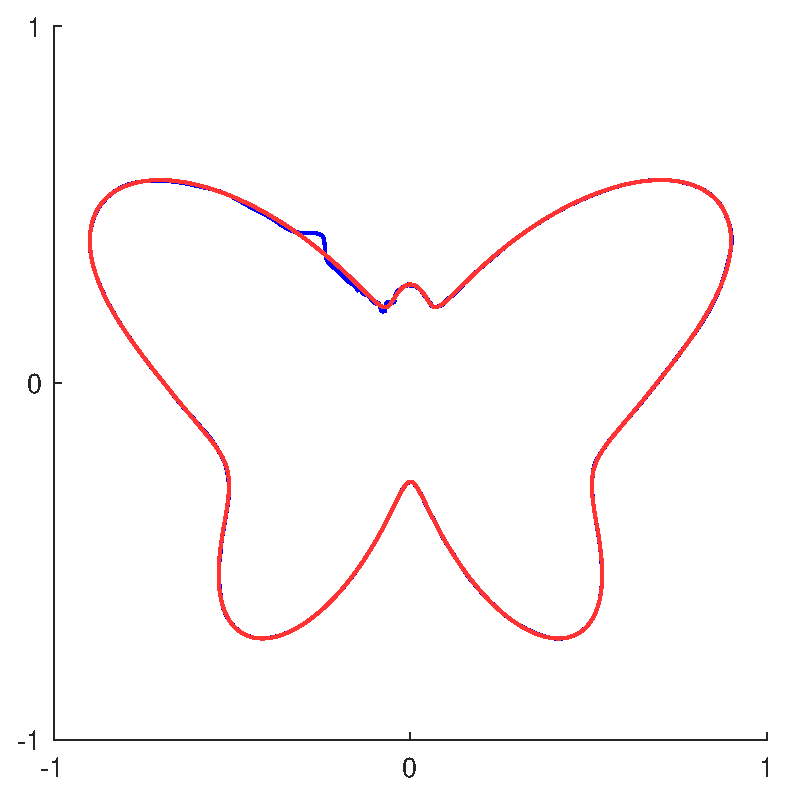
\includegraphics[trim=1.5cm 3cm 1.5cm 3cm, clip=true, height=.2\linewidth]{Figures/Fig_T1/MATLAB/FORCE_T1_Trajectory_axis}
        \includegraphics[trim=1.5cm 2cm 1.5cm 2cm, clip=true,height=.1\textheight]{Figures/Fig_T1/MATLAB/FORCE_T1_Trajectory_noaxis}
        \hspace{3em}
        \includegraphics[height=.08\textheight]{Figures/Fig_T1/Orig/FORCE_T1_Trajectory}
        \hspace{3em}
        \includegraphics[trim=1.5cm 2cm 1.5cm 2cm, clip=true,height=.1\textheight]{Figures/Fig_T1/Python/FORCE_T1_Trajectory_noaxis}

        \end{subfigure}
         
         
        \textbf{\rotatebox[origin=c]{90}{x(t)}}\begin{subfigure}{\textwidth}
        \centering
        
        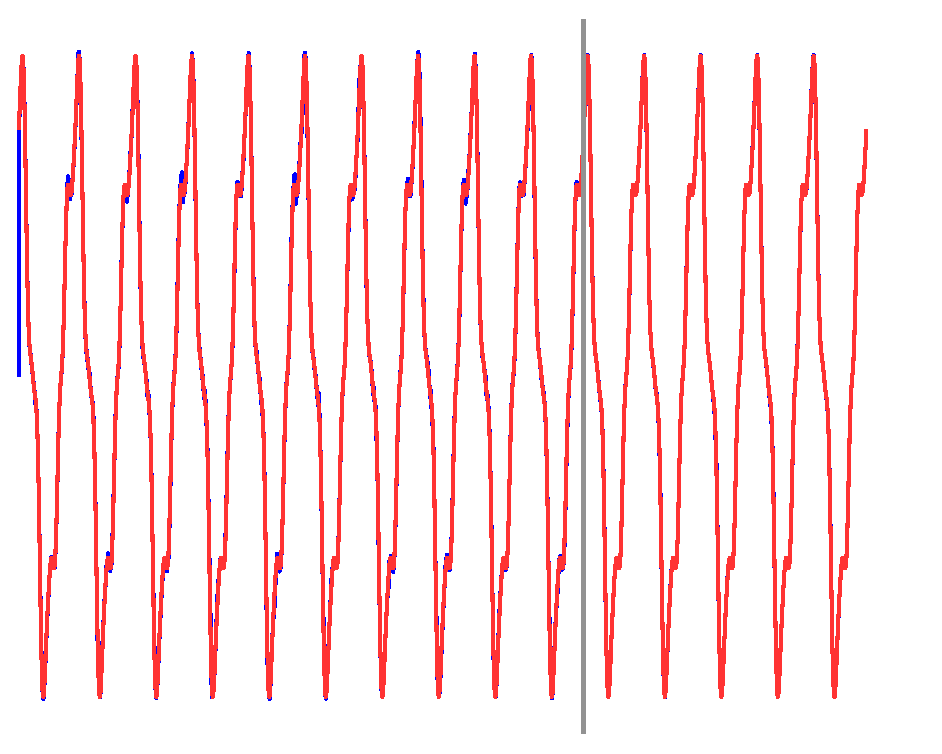
\includegraphics[height=0.08\linewidth,width=.45\linewidth]{Figures/Fig_T1/MATLAB/FORCE_T1_CoordinateX}
        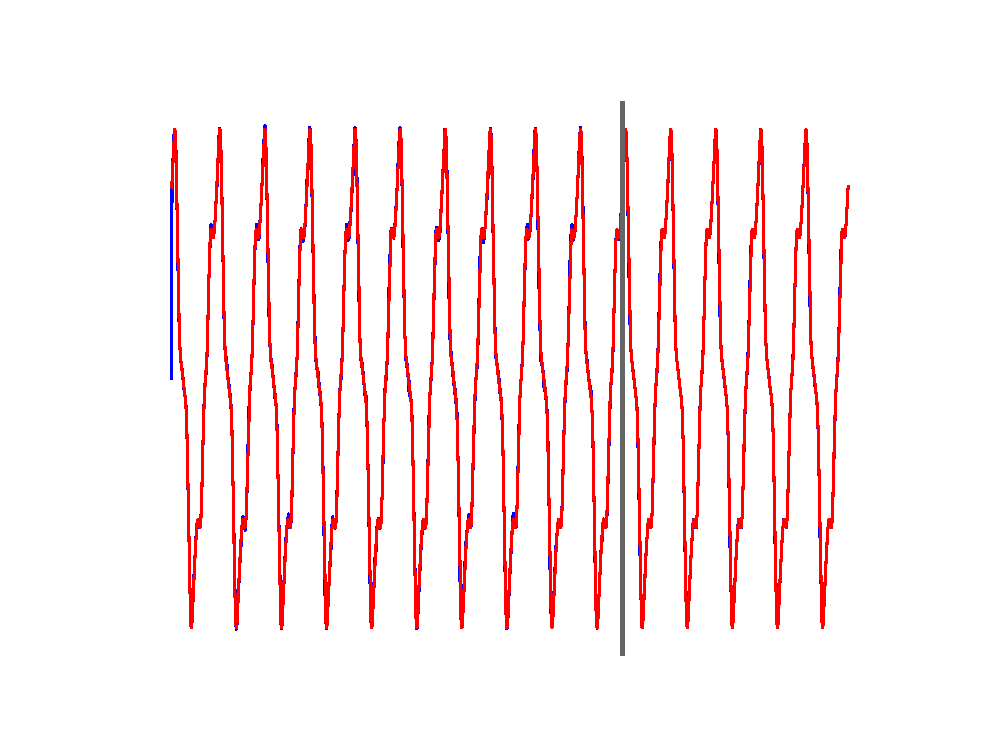
\includegraphics[trim=2cm 1cm 2cm 1cm, clip=true,height=0.08\linewidth,width=.45\linewidth]{Figures/Fig_T1/Python/FORCE_T1_CoordinateX}
        
        \end{subfigure}
        
        
        \textbf{\rotatebox[origin=c]{90}{y(t)}}\begin{subfigure}{\textwidth}
        \centering
        
        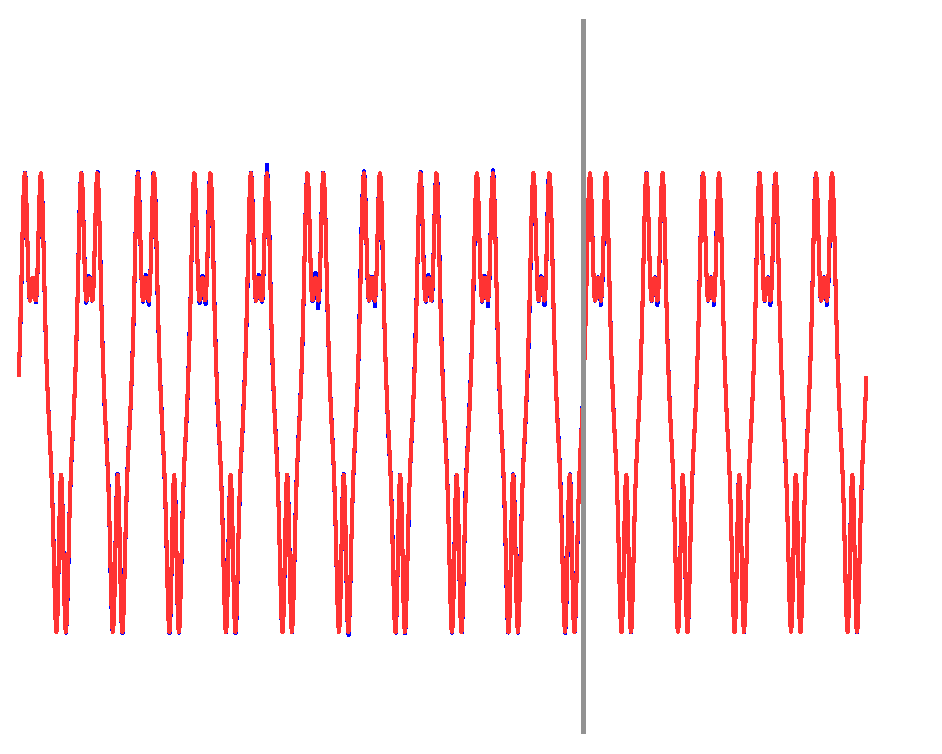
\includegraphics[height=0.08\linewidth,width=.45\linewidth]{Figures/Fig_T1/MATLAB/FORCE_T1_CoordinateY}
        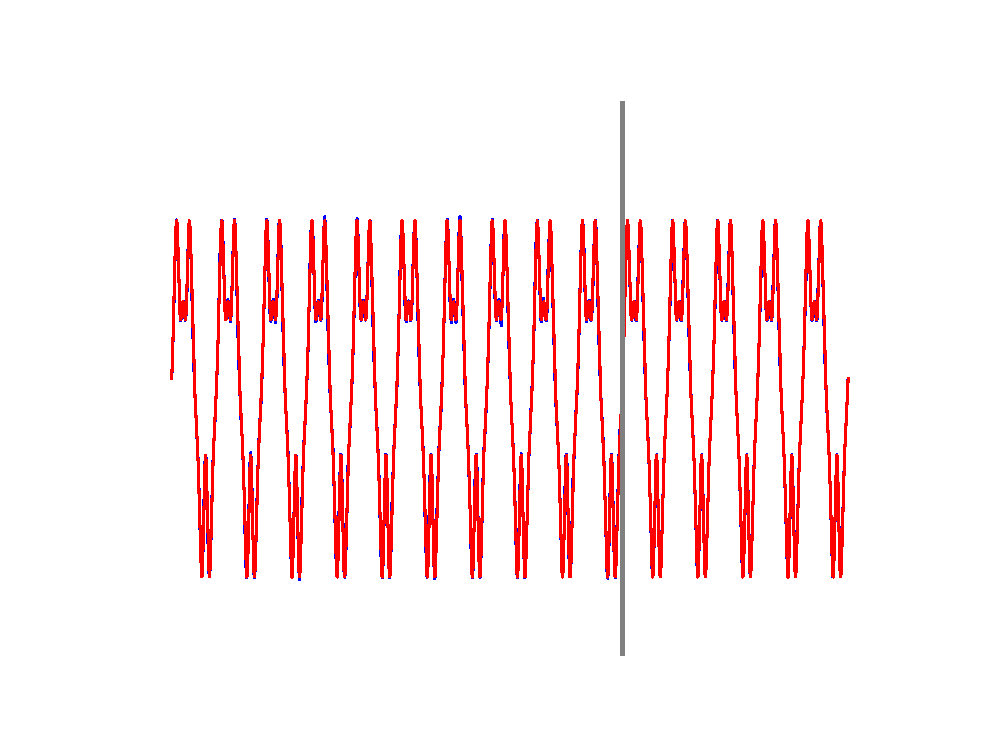
\includegraphics[trim=2cm 1cm 2cm 1cm, clip=true,height=0.08\linewidth,width=.45\linewidth]{Figures/Fig_T1/Python/FORCE_T1_CoordinateY}
        
        \end{subfigure}
        

    \caption{Results for Task 1 with the FORCE algorithm. The target time‐series is learned accurately during the training phase and is maintained in a stable manner during the testing phase, in both implementations, as presented in \cite{pyle2019}.}
    \label{Fig:compTask1FORCE}
    \end{subfigure}

    \begin{subfigure}{\textwidth}
        \centering
        
        \textbf{\rotatebox[origin=c]{90}{RMHL}}\begin{subfigure}{\textwidth}
        \centering
        
        \includegraphics[trim=3cm 4cm 3cm 4cm, clip=true,height=.1\textheight]{Figures/Fig_T1/MATLAB/RHML_T1_Trajectory}
        \hspace{4em}
        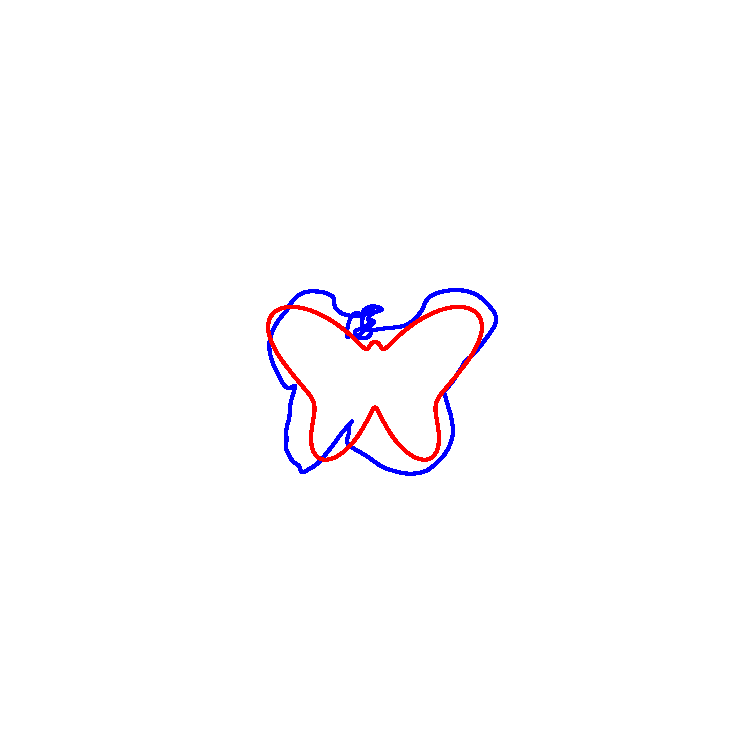
\includegraphics[height=.08\textheight]{Figures/Fig_T1/Orig/RMHL_T1_Trajectory}
        \hspace{4em}
        \includegraphics[trim=6cm 4.5cm 6cm 4.5cm, clip=true,height=.1\textheight]{Figures/Fig_T1/Python/RHML_T1_Trajectory}
        
        \end{subfigure}
         
        
        
        \textbf{\rotatebox[origin=c]{90}{x(t)}}\begin{subfigure}{\textwidth}
        \centering
        
        \includegraphics[height=0.08\linewidth,width=.45\linewidth]{Figures/Fig_T1/MATLAB/RHML_T1_CoordinateX}
        \includegraphics[trim=2cm 1cm 2cm 1cm, clip=true,height=0.08\linewidth,width=.45\linewidth]{Figures/Fig_T1/Python/RHML_T1_CoordinateX}
        
        \end{subfigure}
         
        
        
        \textbf{\rotatebox[origin=c]{90}{y(t)}}\begin{subfigure}{\textwidth}
        \centering
        
        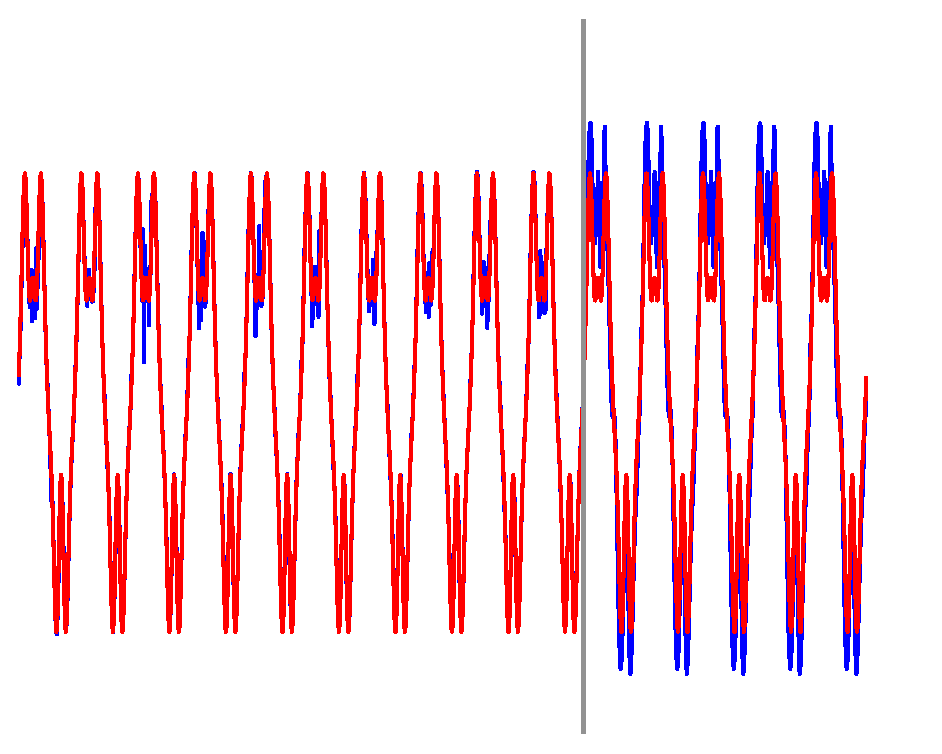
\includegraphics[height=0.08\linewidth,width=.45\linewidth]{Figures/Fig_T1/MATLAB/RHML_T1_CoordinateY}
        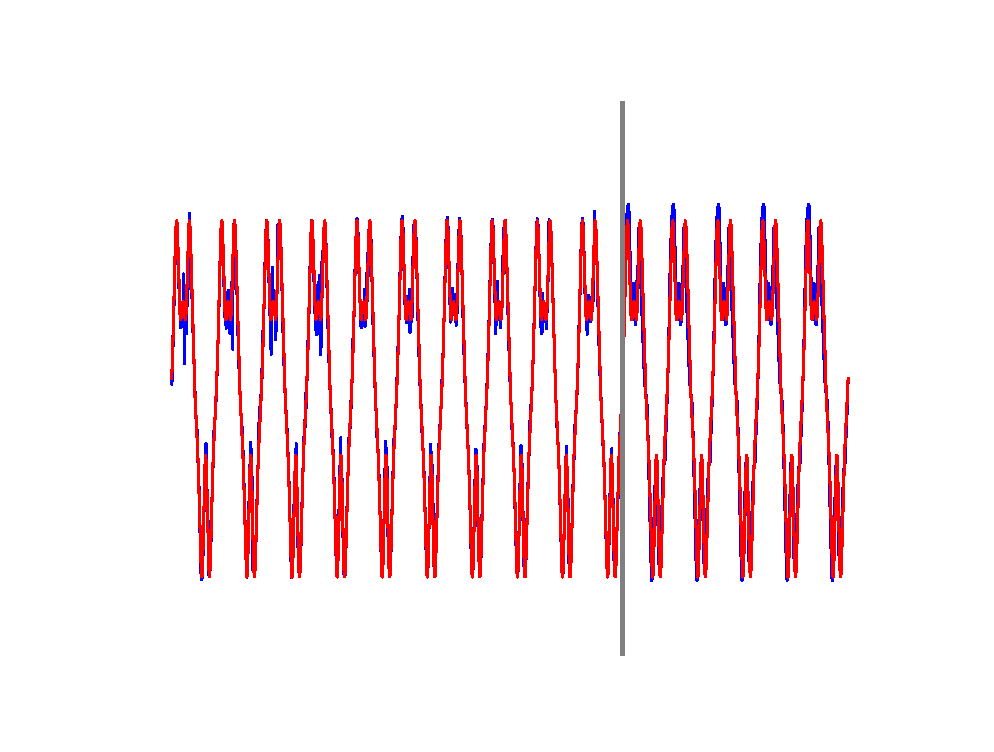
\includegraphics[trim=2cm 1cm 2cm 1cm, clip=true,height=0.08\linewidth,width=.45\linewidth]{Figures/Fig_T1/Python/RHML_T1_CoordinateY}
        
        \end{subfigure}
        
    \caption{Results for Task 1 with the RMHL algorithm. The target time‐series is learned accurately during the training phase, though not maintained perfectly during the testing phase, in both implementations, as presented in \cite{pyle2019}.}
    \label{Fig:compTask1RMHL}
    \end{subfigure}
    
    \begin{subfigure}{\textwidth}
        \centering
        
        \textbf{\rotatebox[origin=c]{90}{SUPERTREX}}\begin{subfigure}{\textwidth}
        \centering
        
        
\includegraphics[trim=3cm 4cm 3cm 4cm, clip=true,height=.1\textheight]{Figures/Fig_T1/MATLAB/ST_T1_Trajectory.eps}
        \hspace{4em}
        
\includegraphics[height=.08\textheight]{Figures/Fig_T1/Orig/ST_T1_Trajectory.png}
        \hspace{4em}
        
\includegraphics[trim=6cm 4.5cm 6cm 4.5cm,clip=true,height=.1\textheight]{Figures/Fig_T1/Python/ST_T1_Trajectory.eps}
        
        \end{subfigure}
         
        
        
        \textbf{\rotatebox[origin=c]{90}{x(t)}}\begin{subfigure}{\textwidth}
        \centering
        
        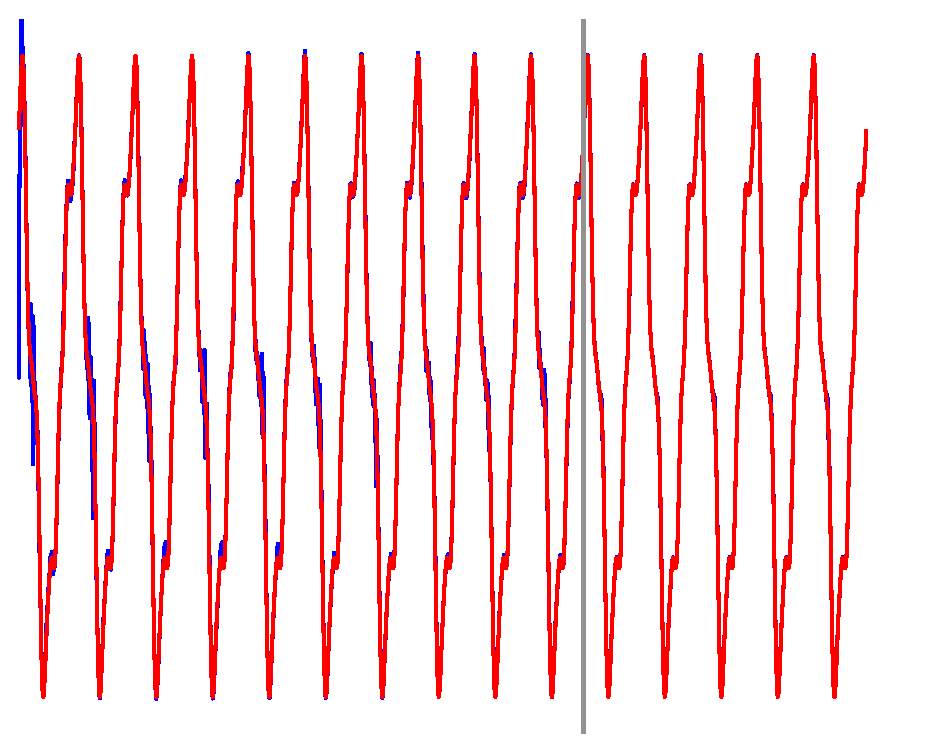
\includegraphics[height=0.08\linewidth,width=.4\linewidth]{Figures/Fig_T1/MATLAB/ST_T1_CoordinateX}
        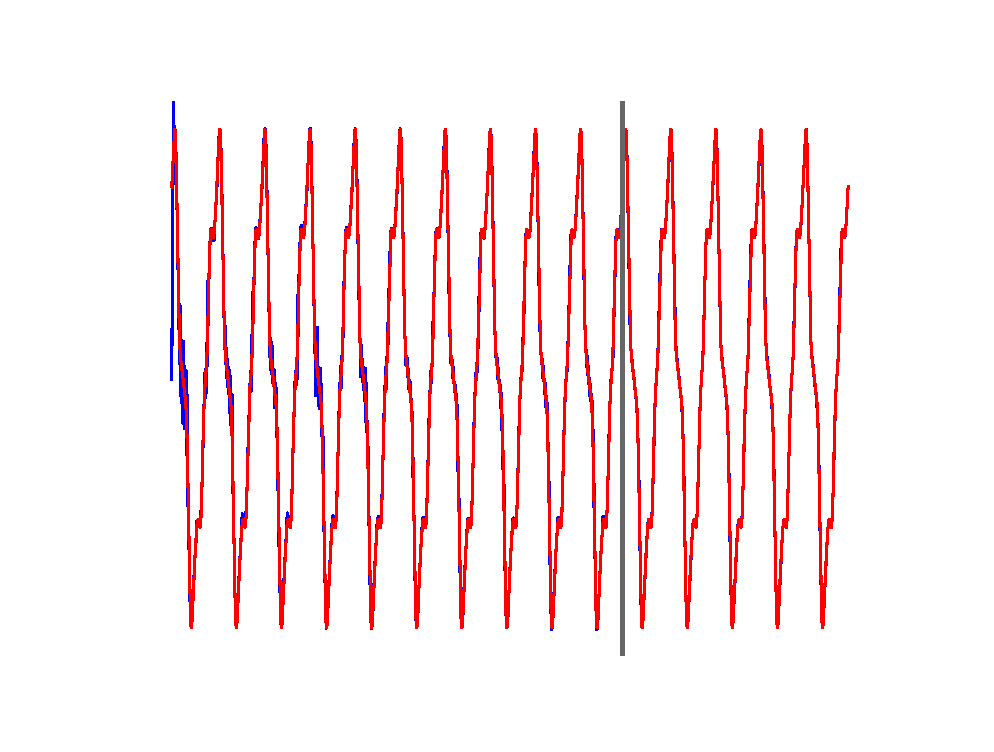
\includegraphics[trim=2cm 1cm 2cm 1cm, clip=true,height=0.08\linewidth,width=.45\linewidth]{Figures/Fig_T1/Python/ST_T1_CoordinateX}
        
        \end{subfigure}
         
        
        
        \textbf{\rotatebox[origin=c]{90}{y(t)}}\begin{subfigure}{\textwidth}
        \centering
        
        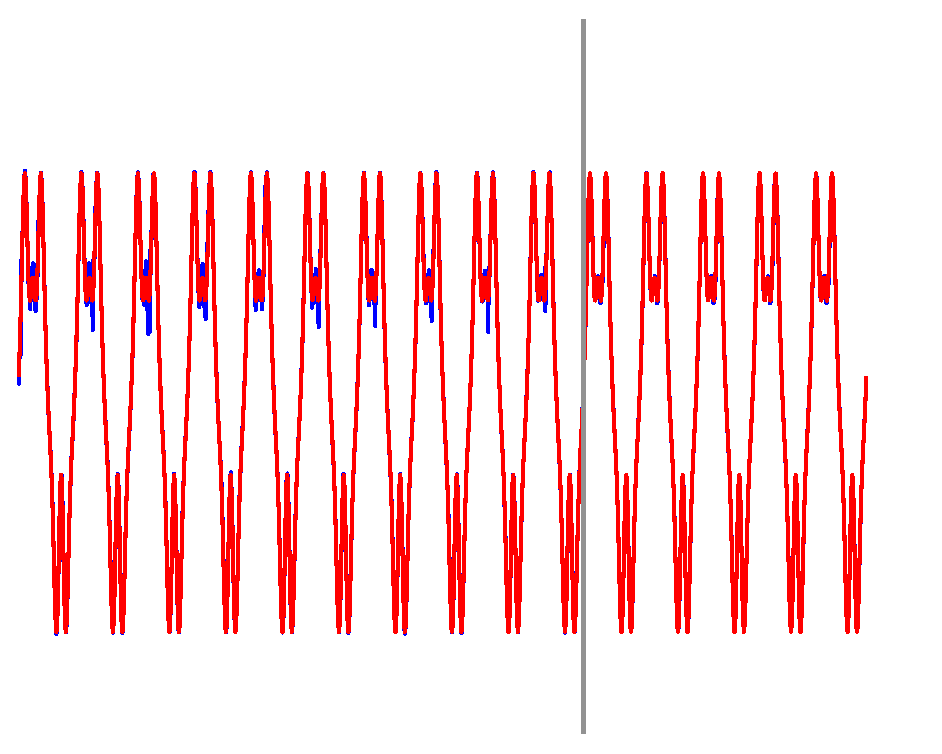
\includegraphics[height=0.08\linewidth,width=.4\linewidth]{Figures/Fig_T1/MATLAB/ST_T1_CoordinateY}
        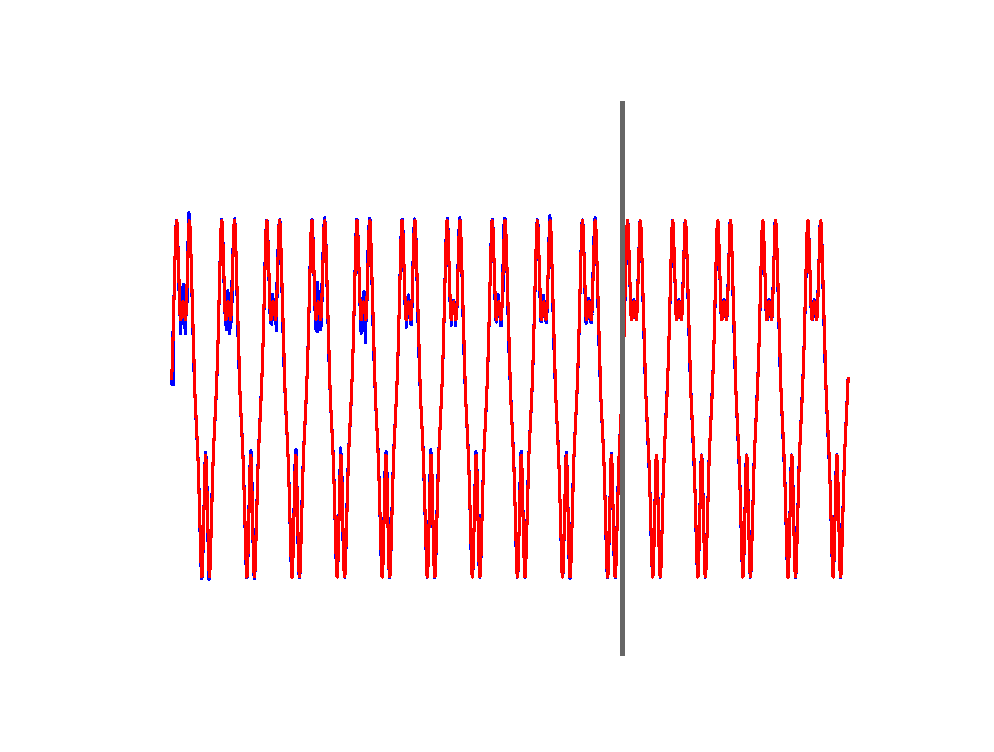
\includegraphics[trim=2cm 1cm 2cm 1cm, clip=true,height=0.08\linewidth,width=.45\linewidth]{Figures/Fig_T1/Python/ST_T1_CoordinateY}
        
        \end{subfigure}
        
        
        
        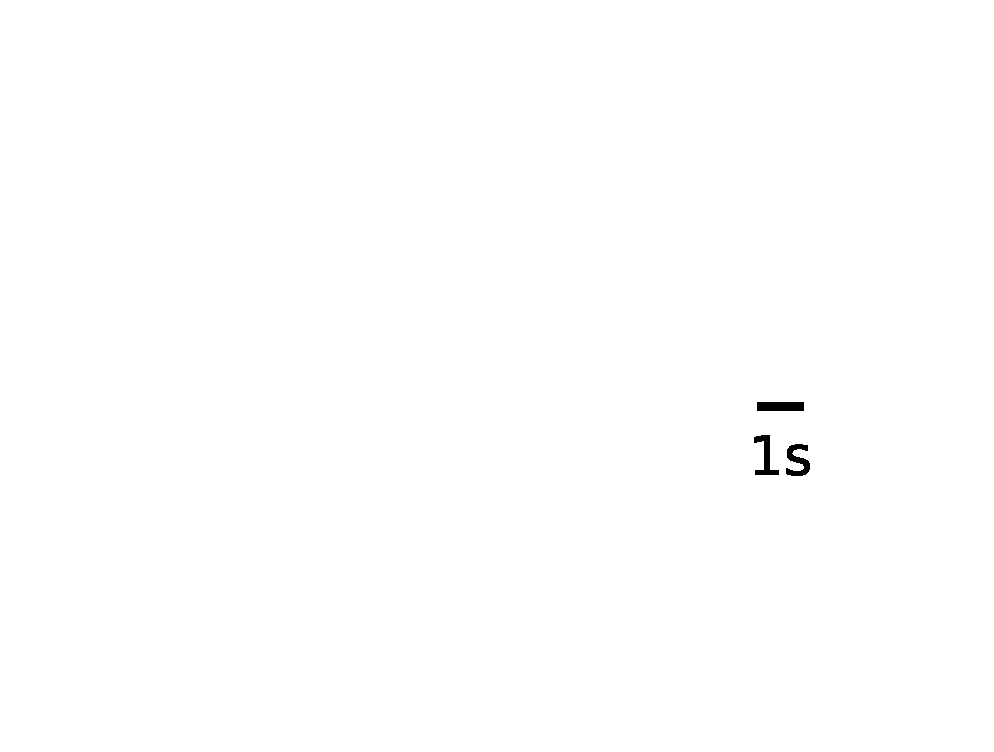
\includegraphics[trim=2cm 6cm 2cm 6cm, clip=true,height=0.05\linewidth,width=.4\linewidth]{Figures/Fig_T1/Python/ST_T1_Scale.eps}
        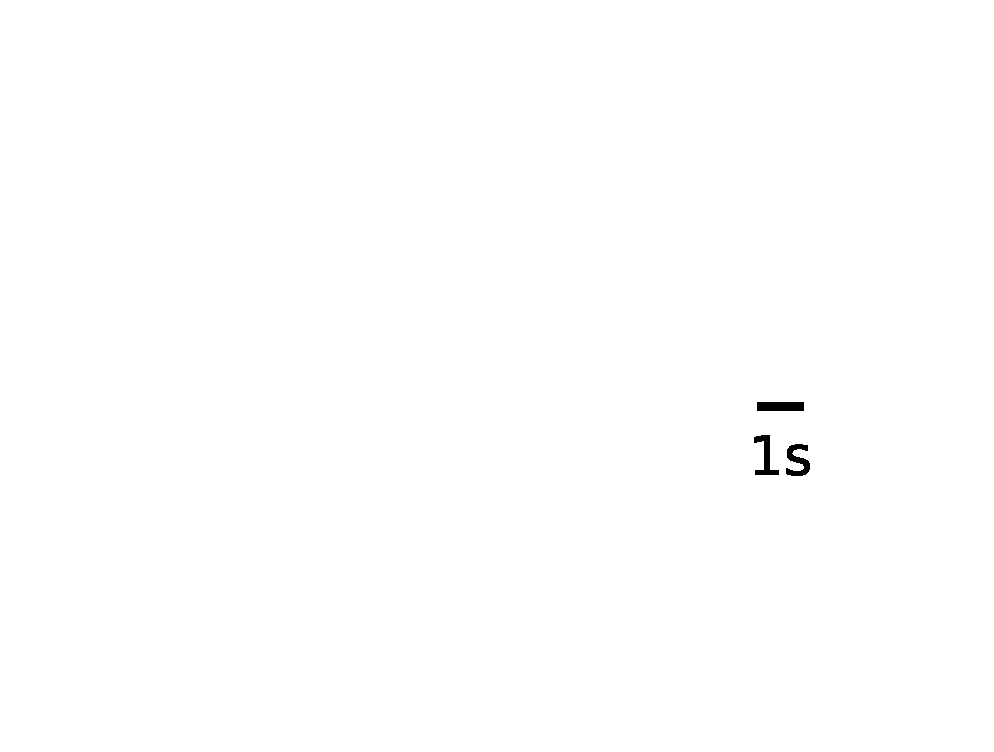
\includegraphics[trim=2cm 4cm 2cm 6cm, clip=true,height=0.05\linewidth,width=.45\linewidth]{Figures/Fig_T1/Python/ST_T1_Scale.eps}
        

    \caption{Results for Task 1 with the SUPERTREX algorithm. The target time‐series is learned accurately during the training phase, and is also maintained in a stable manner during testing phase, albeit not as well as FORCE, in both implementations, as presented in \cite{pyle2019}.}
    \label{Fig:compTask1ST}
    
    \end{subfigure}


\caption{Comparison of the performances of the MATLAB scripts (left column) and the Python adaptation (right column) with the results presented in the original article (center column), for the three learning algorithms on Task 1 \cite{pyle2019}. All simulations shown here use the MATLAB default (5489) as the seed for the random number generator. In each subfigure, the top row shows the target trajectory (red) with the trajectory generated by the model (blue) throughout the test phase. The second row shows the time-series (blue) generated by the model (x and y coordinates, in this case) along with the target time-series (red). The grey vertical line marks the separation of the training and testing phase.}
\label{Fig:Comparison_Task1}

\end{figure}


\begin{figure}

    \centering
    \textbf{MATLAB}\hspace{8em}
    \textbf{Original}\hspace{8em}
    \textbf{Python}
    
    \begin{subfigure}{\textwidth}
        \centering
        
        \textbf{\rotatebox[origin=c]{90}{FORCE}}\begin{subfigure}{\textwidth}
        \centering
    
        \includegraphics[trim=1.5cm 2cm 1.5cm 2cm, clip=true,height=.1\textheight]{Figures/Fig_T1/MATLAB/FORCE_T1_Trajectory_noaxis}
        \hspace{3em}
        \includegraphics[height=.08\textheight]{Figures/Fig_T1/Orig/FORCE_T1_Trajectory}
        \hspace{3em}
        \includegraphics[trim=1.5cm 2cm 1.5cm 2cm, clip=true,height=.1\textheight]{Figures/Fig_T1/Python/FORCE_T1_Trajectory_noaxis}

        \end{subfigure}
         
         
        \textbf{\rotatebox[origin=c]{90}{MSE}}\begin{subfigure}{\textwidth}
        \centering
        
        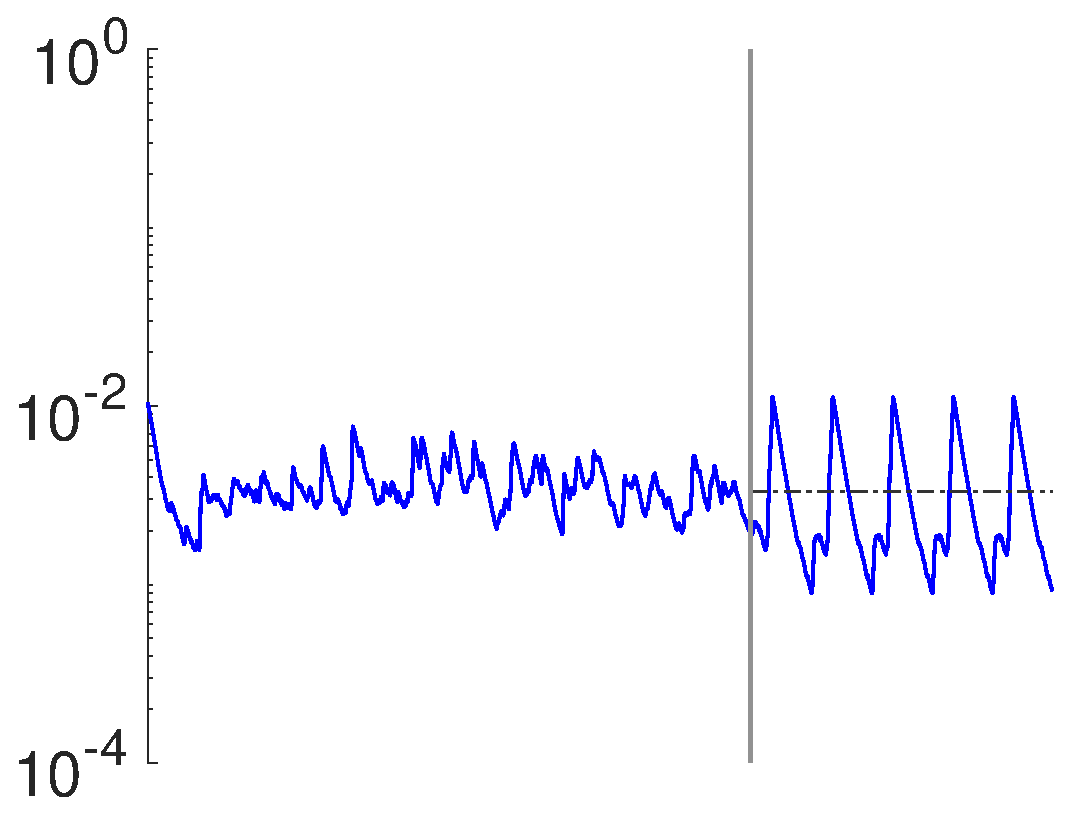
\includegraphics[height=0.12\linewidth,width=.45\linewidth]{Figures/Fig_T1/MATLAB/FORCE_T1_MSE.eps}
        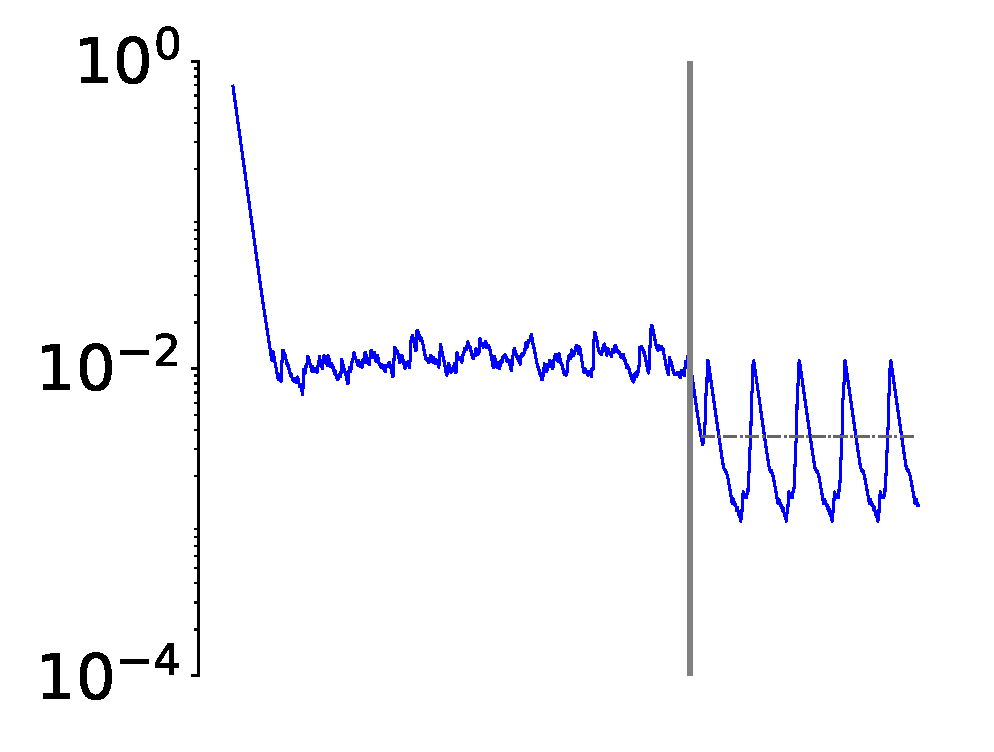
\includegraphics[height=0.12\linewidth,width=.45\linewidth]{Figures/Fig_T1/Python/FORCE_T1_MSE.eps}
        
        \end{subfigure}
        
        
        \textbf{\rotatebox[origin=c]{90}{||W||}}\begin{subfigure}{\textwidth}
        \centering
        
        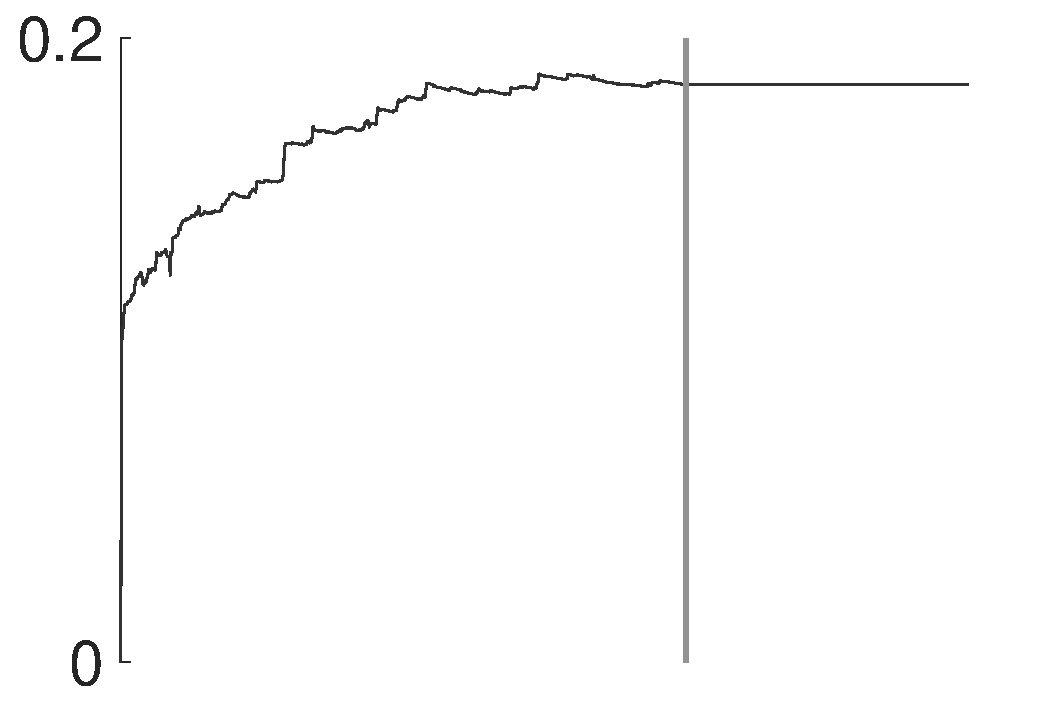
\includegraphics[trim=0cm 0cm 1cm 0cm, clip=true,height=0.12\linewidth,width=.45\linewidth]{Figures/Fig_T1/MATLAB/FORCE_T1_W_norm.eps}
        \hspace{.3em}
        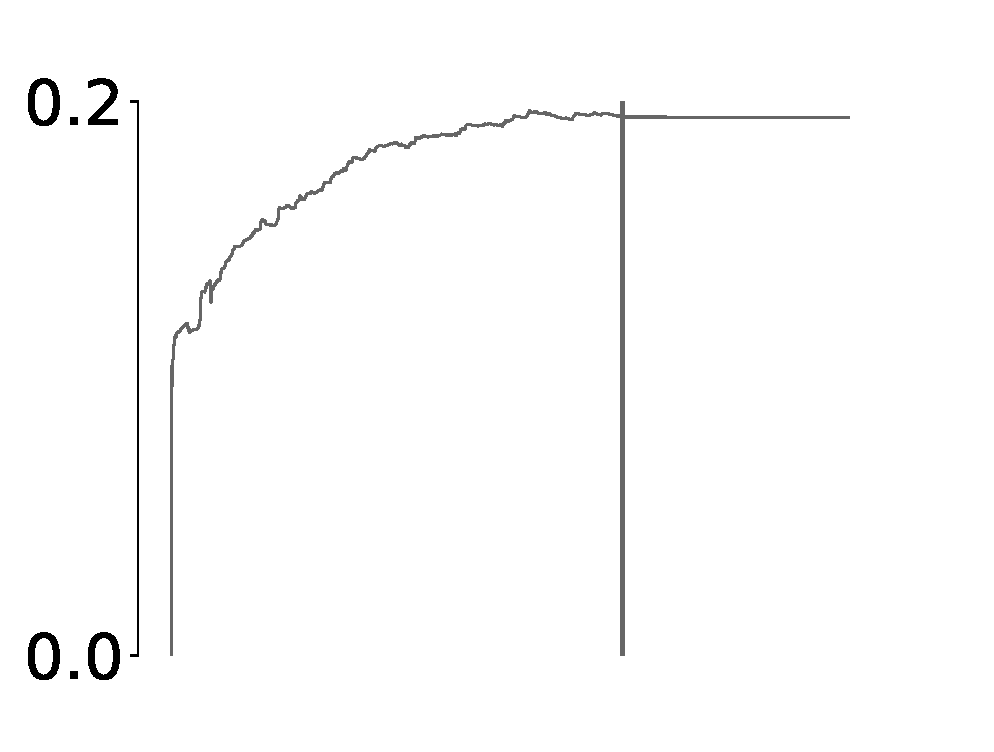
\includegraphics[trim=0cm 0cm 1cm 0cm, clip=true,height=0.12\linewidth,width=.45\linewidth]{Figures/Fig_T1/Python/FORCE_T1_W_norm.eps}
        
        \end{subfigure}
        

    \caption{Results for Task 1 with the FORCE algorithm. The target time‐series is learned accurately during the training phase and is maintained in a stable manner during the testing phase, as presented in \cite{pyle2019}.}
    \label{Fig:compTask1FORCE_MSE}
    \end{subfigure}

    \begin{subfigure}{\textwidth}
        \centering
        
        \textbf{\rotatebox[origin=c]{90}{RMHL}}\begin{subfigure}{\textwidth}
        \centering
        
        \includegraphics[trim=3cm 4cm 3cm 4cm, clip=true,height=.1\textheight]{Figures/Fig_T1/MATLAB/RHML_T1_Trajectory}
        \hspace{4em}
        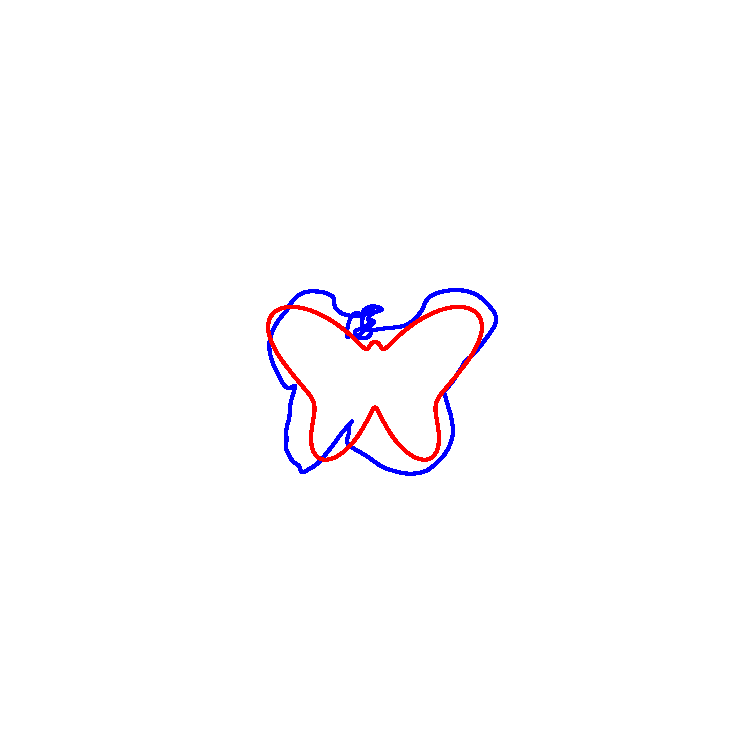
\includegraphics[height=.08\textheight]{Figures/Fig_T1/Orig/RMHL_T1_Trajectory}
        \hspace{4em}
        \includegraphics[trim=6cm 4.5cm 6cm 4.5cm, clip=true,height=.1\textheight]{Figures/Fig_T1/Python/RHML_T1_Trajectory}
        
        \end{subfigure}
         
        
        
        \textbf{\rotatebox[origin=c]{90}{MSE}}\begin{subfigure}{\textwidth}
        \centering
        
        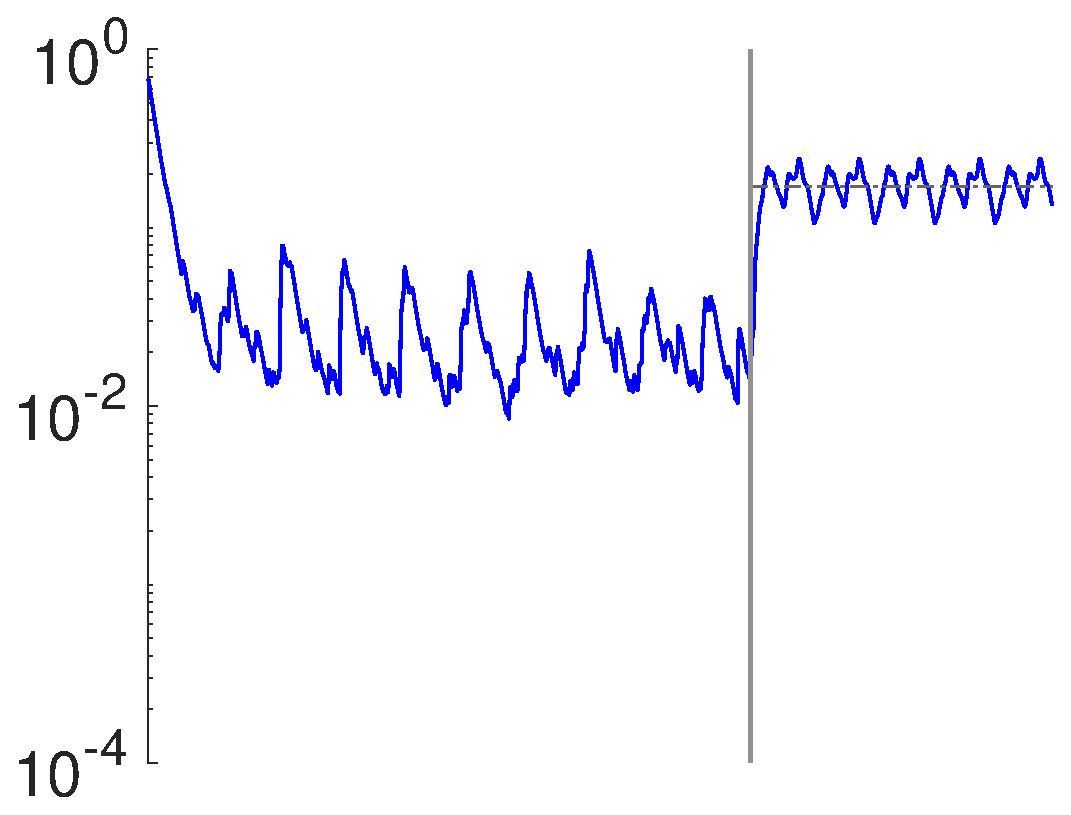
\includegraphics[height=0.12\linewidth,width=.45\linewidth]{Figures/Fig_T1/MATLAB/RHML_T1_MSE.eps}
        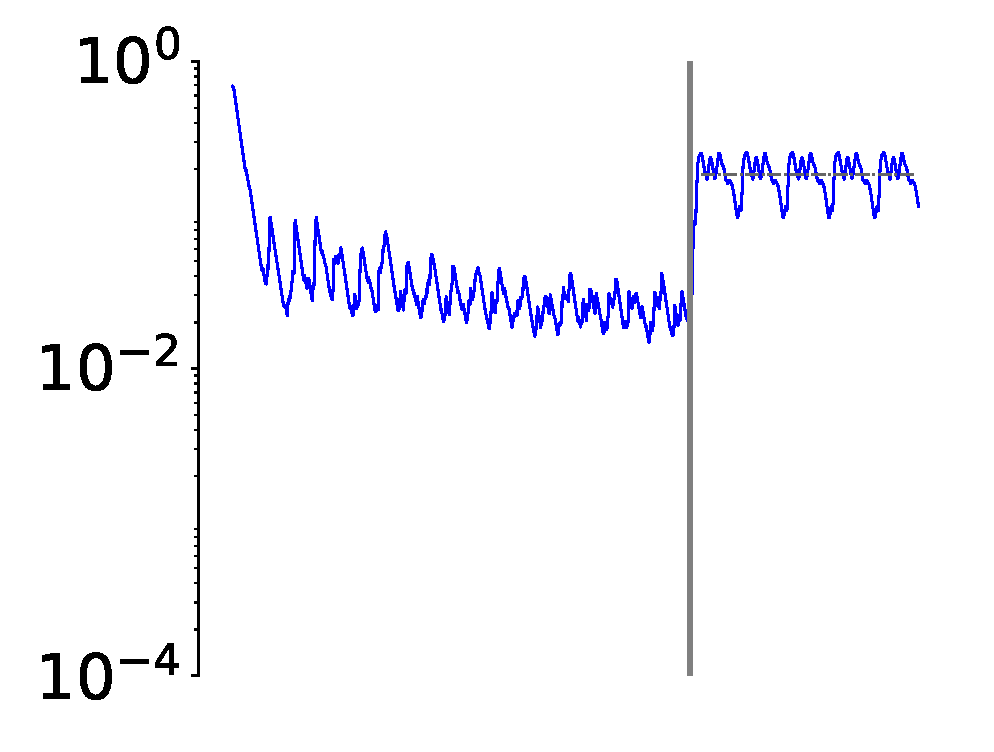
\includegraphics[height=0.12\linewidth,width=.45\linewidth]{Figures/Fig_T1/Python/RHML_T1_MSE.eps}
        
        \end{subfigure}
        
        
        \textbf{\rotatebox[origin=c]{90}{||W||}}\begin{subfigure}{\textwidth}
        \centering
        
        \includegraphics[trim=0cm 0cm 1cm 0cm, clip=true,height=0.12\linewidth,width=.45\linewidth]{Figures/Fig_T1/MATLAB/RHML_T1_W_norm.eps}
        \hspace{.3em}
        \includegraphics[trim=0cm 0cm 1cm 0cm, clip=true,height=0.12\linewidth,width=.45\linewidth]{Figures/Fig_T1/Python/RHML_T1_W_norm.eps}
        
        \end{subfigure}
        
    \caption{Results for Task 1 with the RMHL algorithm. The target time‐series is learned accurately during the training phase, though not maintained perfectly during the testing phase, as presented in \cite{pyle2019}.}
    \label{Fig:compTask1RMHL_MSE}
    \end{subfigure}
    
    \begin{subfigure}{\textwidth}
        \centering
        
        \textbf{\rotatebox[origin=c]{90}{SUPERTREX}}\begin{subfigure}{\textwidth}
        \centering
        
        
\includegraphics[trim=3cm 4cm 3cm 4cm, clip=true,height=.1\textheight]{Figures/Fig_T1/MATLAB/ST_T1_Trajectory.eps}
        \hspace{4em}
        
\includegraphics[height=.08\textheight]{Figures/Fig_T1/Orig/ST_T1_Trajectory.png}
        \hspace{4em}
        
\includegraphics[trim=6cm 4.5cm 6cm 4.5cm,clip=true,height=.1\textheight]{Figures/Fig_T1/Python/ST_T1_Trajectory.eps}
        
        \end{subfigure}
        
        \textbf{\rotatebox[origin=c]{90}{MSE}}\begin{subfigure}{\textwidth}
        \centering
        
        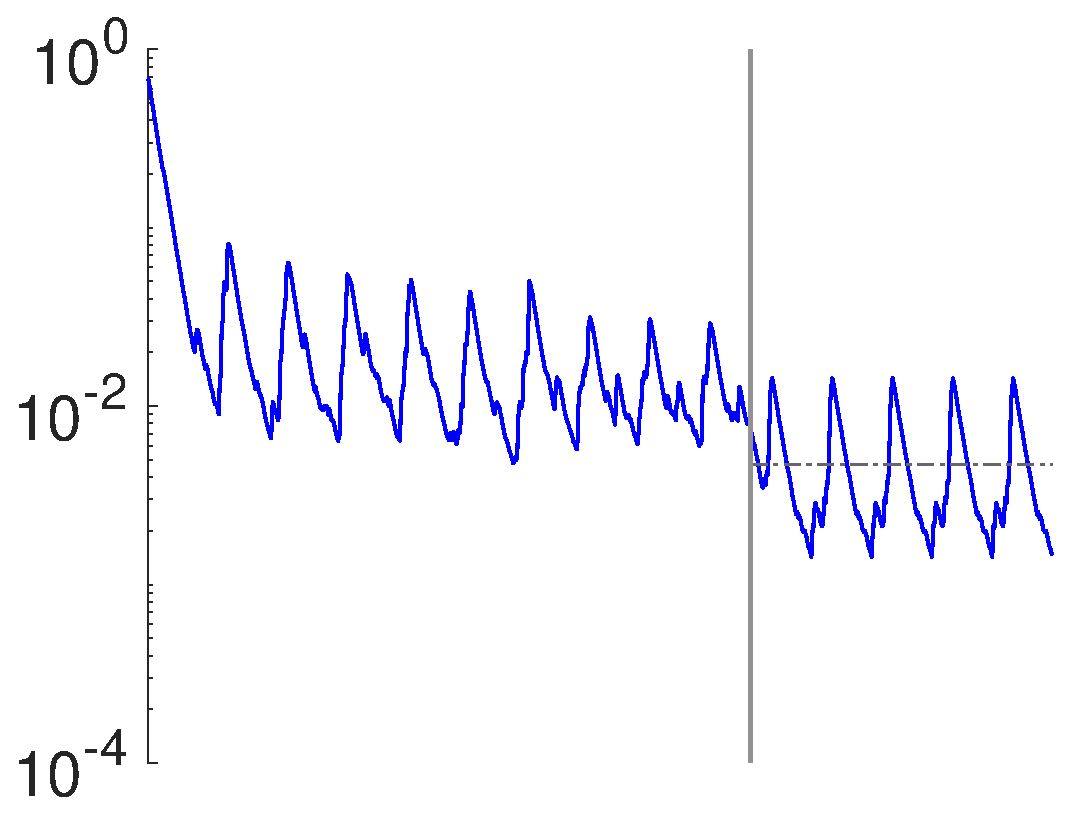
\includegraphics[height=0.12\linewidth,width=.45\linewidth]{Figures/Fig_T1/MATLAB/ST_T1_MSE.eps}
        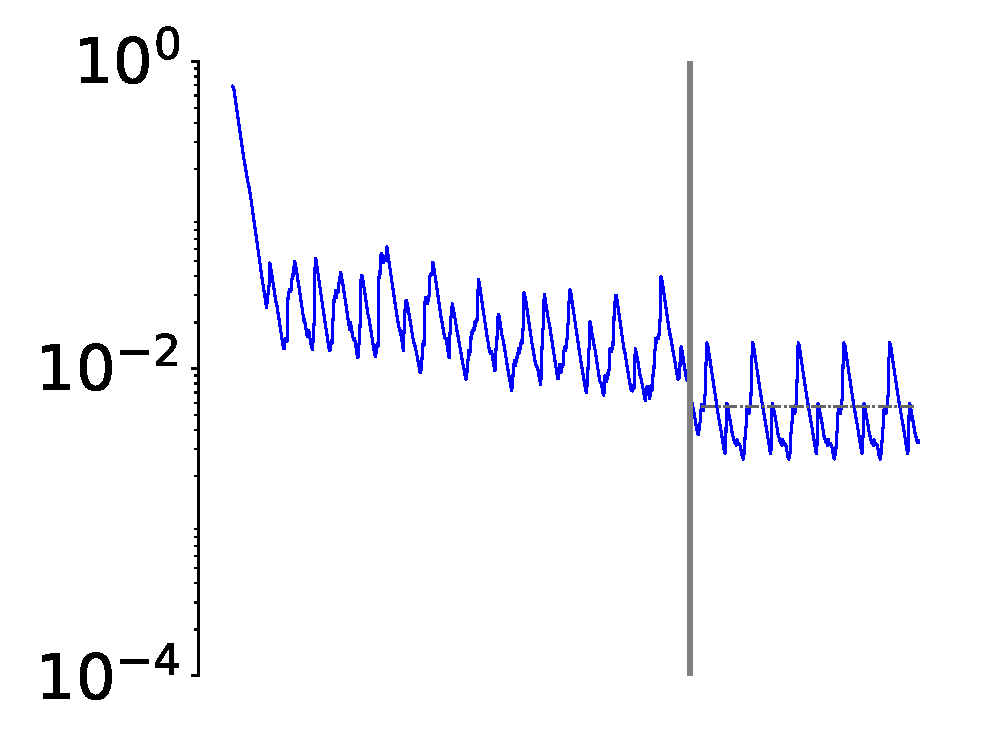
\includegraphics[height=0.12\linewidth,width=.45\linewidth]{Figures/Fig_T1/Python/ST_T1_MSE.eps}
        
        \end{subfigure}
        
        
        \textbf{\rotatebox[origin=c]{90}{||W||}}\begin{subfigure}{\textwidth}
        \centering
        
        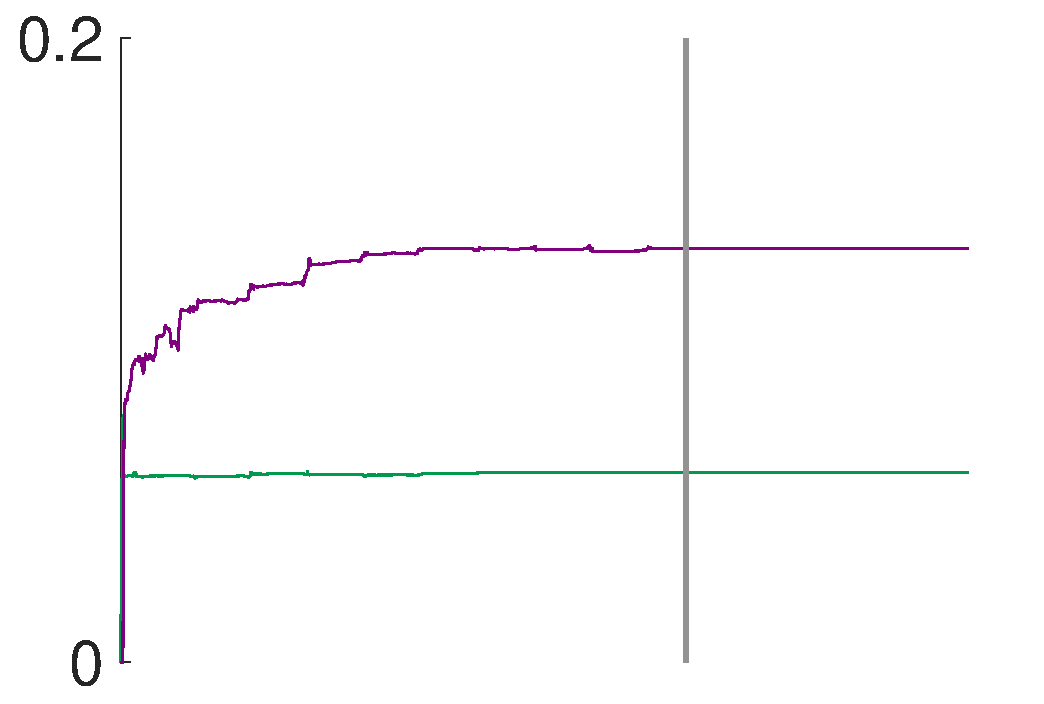
\includegraphics[trim=0cm 0cm 1cm 0cm, clip=true,height=0.12\linewidth,width=.45\linewidth]{Figures/Fig_T1/MATLAB/ST_T1_W_norm.eps}
        \hspace{.3em}
        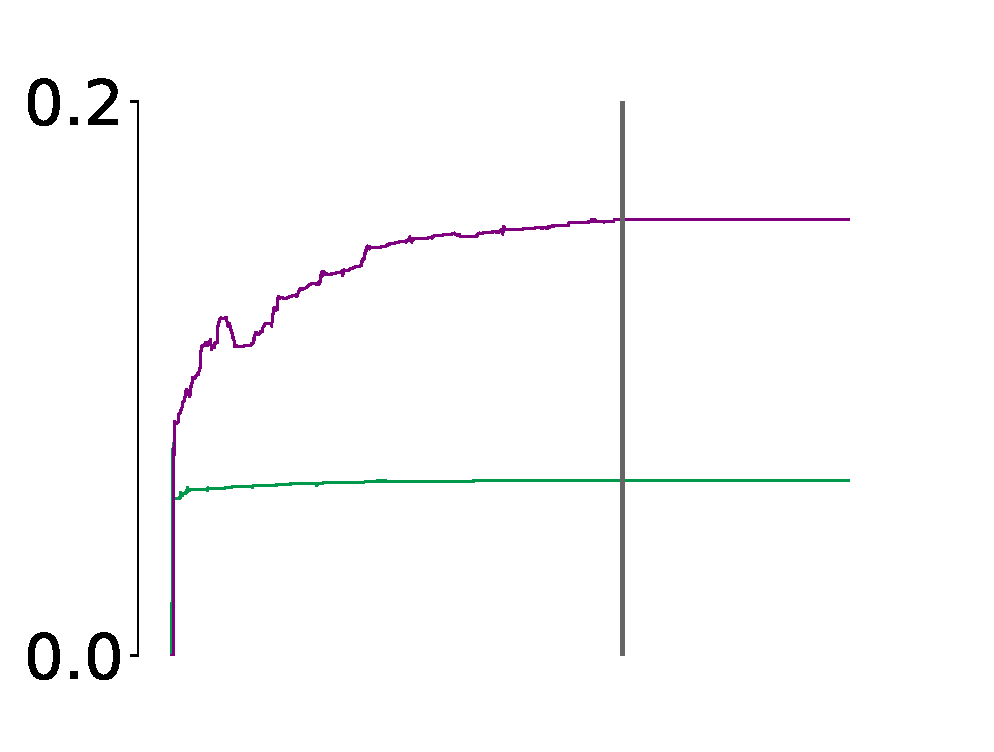
\includegraphics[trim=0cm 0cm 1cm 0cm, clip=true,height=0.12\linewidth,width=.45\linewidth]{Figures/Fig_T1/Python/ST_T1_W_norm.eps}
        
        \end{subfigure}


        
        
        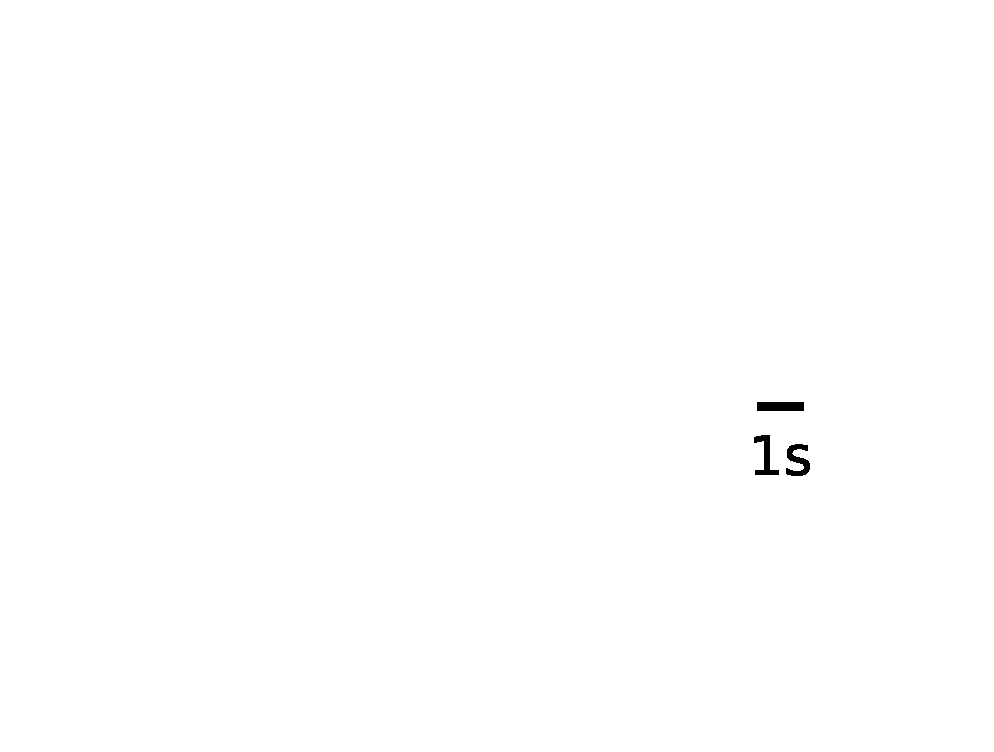
\includegraphics[trim=2cm 6cm 2cm 6cm, clip=true,height=0.05\linewidth,width=.4\linewidth]{Figures/Fig_T1/Python/ST_T1_Scale.eps}
        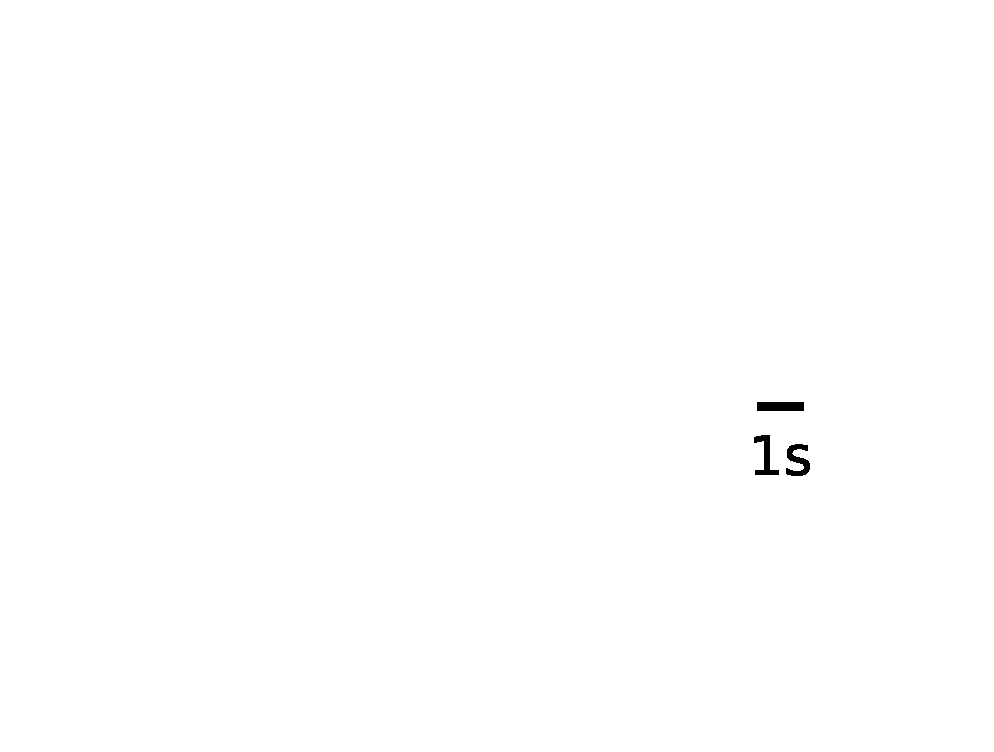
\includegraphics[trim=2cm 4cm 2cm 6cm, clip=true,height=0.05\linewidth,width=.45\linewidth]{Figures/Fig_T1/Python/ST_T1_Scale.eps}
        

    \caption{Results for Task 1 with the SUPERTREX algorithm. The target time‐series is learned accurately during the training phase, and is also maintained in a stable manner during testing phase, albeit not as well as FORCE, as presented in \cite{pyle2019}.}
    \label{Fig:compTask1ST_MSE}
    
    \end{subfigure}


\caption{Comparison of the performances of the MATLAB scripts (left column) and the Python adaptation (right column) with the results presented in the original article (center column), for the three learning algorithms on Task 1 \cite{pyle2019}. All simulations shown here use the MATLAB default (5489) as the seed for the random number generator. In each subfigure, the top row shows the target trajectory (red) with the trajectory generated by the model (blue) throughout the test phase. The second row shows the error metric (blue) over the simulation (x and y coordinates, in this case), using the log scale for the y axis. The bottom row shows the progression of the corresponding weight matrices (SUPERTREX: $W_1$ in purple; $W_2$, in green). The horizontal grey line, in the test phase, indicates the deviation metric.}
\label{Fig:Comparison_Task1_MSE}

\end{figure}

